\section{Pics Manager - Make}
%The similarities with Profile Pics Changer
The way the Pics Manager - Make feature is implemented is very similar to how the Profile Picture Changer is implemented, see section \ref{sec:profilePicChange}.\\
They both get called the same way and both rely on the HTML Form Element to receive their data. They also give back their error message in the same way.\\
\\
%The special user interface
But what is more interesting is their differences. Looking at figure \ref{fig:picsManagerMake} it can be seen how the user interface is designed. The top left part is for entering the general data, and the right side is for the image and the sound file.\\
\\
We have designed it so that when a user chooses a sound file, or an image file, they can hear, or see, a preview of it before uploading. We also did this so that the design could be reused for the editing feature.\\
The preview is possible because of a JavaScript function called \texttt{FileReader}. Which simply loads the file into the browser, and makes it possible to work with it without uploading the file. But this is only available in some of the newer browsers. Which means we have had to disregard the use of IE9 \citep{canIUse}. In doing so we have created a warning on our login screen that checks if the \texttt{FileReader} is available, and if not the user will be meet with a warning, telling them some features will not function for them.\\
\\
\begin{figure}[htbp]
	\centering
		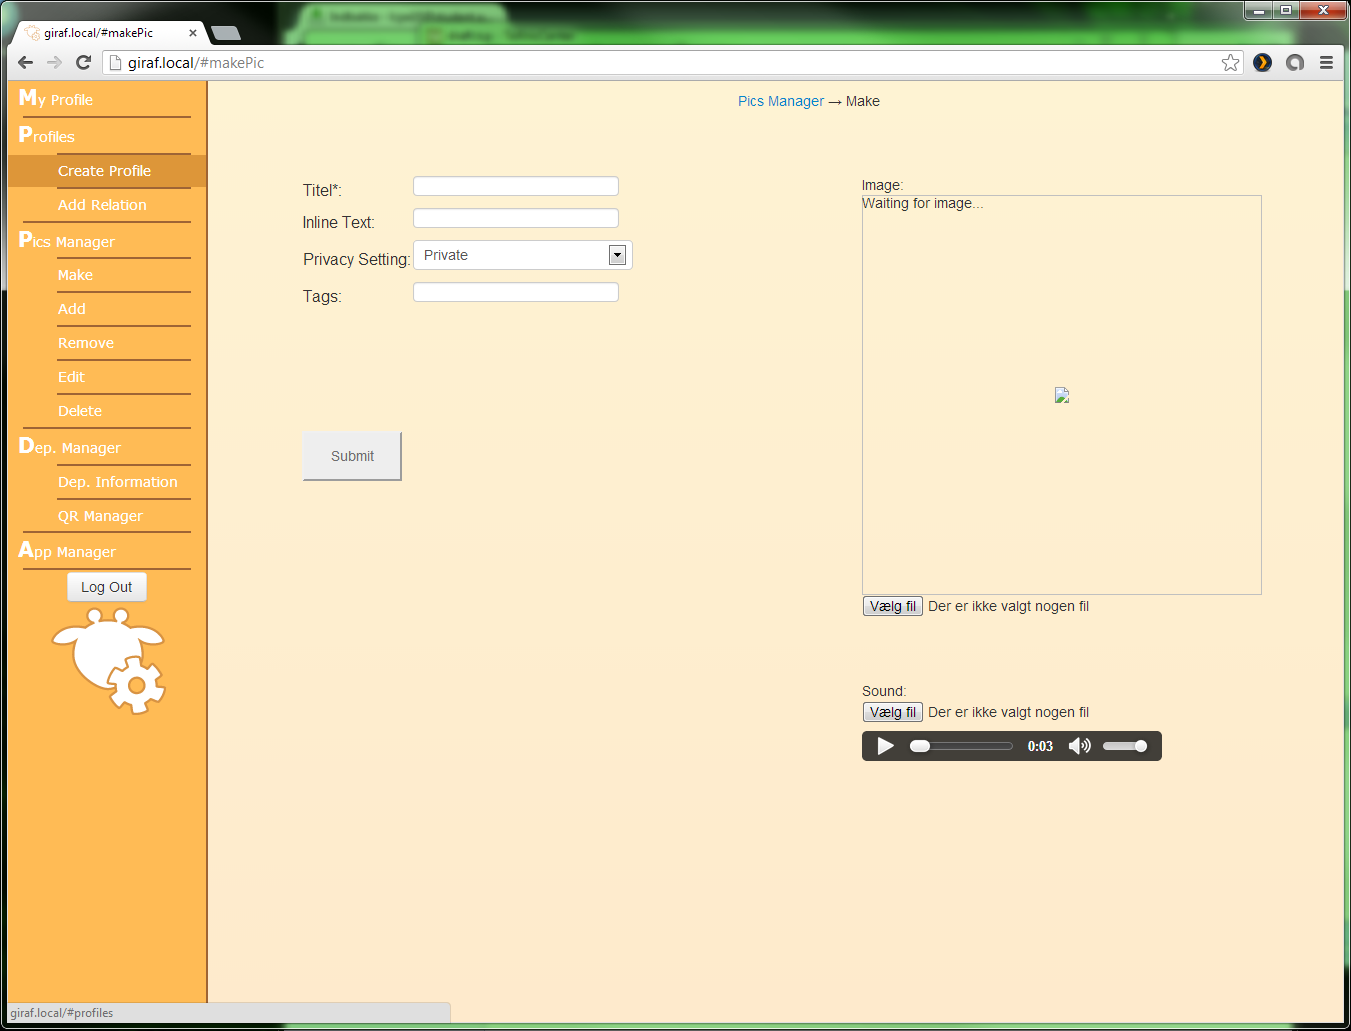
\includegraphics[width=1\textwidth]{images/picsManagerMake.png}
	\caption{The user interface for the Pics Manager - Make}
	\label{fig:picsManagerMake}
\end{figure}

%The special sound file recognizer
Again when speaking about the backend of this feature, it is very similar to the Profile Picture Changer Feature, where the main difference is that Pics Manager - Make has a specialized sound file recognizer, since this is not natively supported in PHP.\\
The function used for this can be seen in listing \ref{lst:soundFileRecognizer}, the first 2 lines (L. 2-3) creates two arrays, one for accepted mime-types and the other for accepted file extensions.\\
Next we do the actual check on file extension and mime-type. (L. 6-23), this is done by simply pulling out the information from the uploaded sound file, and see if it matches any of the variants in the arrays. This do mean that the user can upload a file with a \texttt{mp3} mime-type and a \texttt{.wav} file extension. - But since this is still an accepted sound file it is no security risk.\\
As it can be seen we use two variables which is used as booleans, \texttt{\$fileExtOkay} and \texttt{\$fileMimeTypeOkay}, these are used when we want to return the information of whether or not this was an acceptable sound file (L. 26-31).

\lstset{language=PHP}
\begin{figure}[htbp]
\begin{lstlisting}[firstline=1]
	function isAllowedSoundFile($fileName,$fileTmpName){
		$supportedExtensions = array('3gp','3gpp','flac','mp3','mid','xmf','mxmf','rtttl','rtx','ota','imy','ogg','wav');
		$supportedMimeTypes = array('audio/mpeg','audio/mp3','audio/mid','audio/wav','audio/x-wav','audio/rtx','audio/3gpp','audio/ogg','audio/mobile-xmf','audio/mxf'); //Could not find mime type of .rtttl, .ota and .imy
		
		//Check file extension
		$ext = pathinfo($fileName, PATHINFO_EXTENSION);
		if(in_array($ext,$supportedExtensions)){
			$fileExtOkay = true;
		}
		else{
			$fileExtOkay = false;
		}
		
		//Check Mime Type
		$finfo = finfo_open(FILEINFO_MIME_TYPE); // return mime type ala mimetype extension
		
		if(in_array(finfo_file($finfo, $fileTmpName),$supportedMimeTypes)){
			$fileMimeTypeOkay = true;
		}
		else{
			$fileMimeTypeOkay = false;
		}
		finfo_close($finfo);
		
		//return
		if($fileMimeTypeOkay && $fileExtOkay){
			return true;
		}
		else{
			return false;
		}
	}
\end{lstlisting}
\caption{The function used for checking sound files.}
\label{lst:soundFileRecognizer}
\end{figure}

%The DB query
	%64bit encoding

When the sound and image file have been verified they are sent on to the database query, the main part can be seen at listing \ref{lst:picsManagerMakeDbQuery}. But as also can be seen it is called with a JSON object, which we have another function for. It simply constructs a JSON string from what information the user sent us, we call this function \texttt{makeJsonPictogram}.\\
When we use the function \texttt{makeJsonPictogram} the image and the sound file is encrypted to 64 bit, which is needed in order to ensure we do not mess up the actual database query, not just the JSON object we call the WASTELAND system with. This can be done natively in PHP.\\
\\

\lstset{language=PHP}
\begin{figure}[htbp]
\begin{lstlisting}[firstline=1]
function db_uploadePictogram($jsonPictogram){
	global $session,$username,$password;
	$data = '{
		"action": "create",
		"auth": {
			"username": "'.$username.'",
			"password": "'.$password.'"
		},
	    "data": {
	    	"type":"pictogram",
	    	"values":['.$jsonPictogram.']
	    }
	}';
	
	$result = db_query($data);

	if ($result['status'] == 'OK')
	{
		return $result['data'];
	}
	else
	{
		return false;
	}
}
\end{lstlisting}
\caption{The main part of the DB query for creating Pictograms}
\label{lst:picsManagerMakeDbQuery}
\end{figure}

When the database query have been completed, the feature will as the Profile Picture Changer, send the user to the creation page with a message of success.\\
\\

%Rounding off the implementation chapter
This is the end of all the advanced and complicated solutions we have managed to complete, the next chapter will focus on the results of our usability testing of the somewhat finished system.